\documentclass[hidelinks]{article}

\usepackage[sensei=Ze\ Chen,gakka=Magnetochemistry,section=Magnetochemistry,gakkabbr=MS]{styles/kurisuen}
\usepackage{sidenotes}
\usepackage{van-de-la-sehen-en}
\usepackage{van-de-environnement-en}
\usepackage{boite/van-de-boite-en}
\usepackage{van-de-abbreviation}
\usepackage{van-de-neko}
\usepackage{van-le-trompe-loeil}
\usepackage{cyanide/van-de-cyanide}
\setlength{\parindent}{0pt}
\usepackage{enumitem}
\newlist{citemize}{itemize}{3}
\setlist[citemize,1]{noitemsep,topsep=0pt,label={-},leftmargin=1em}

\usepackage{mathtools}
\usepackage{ragged2e}

\DeclarePairedDelimiter\abs{\lvert}{\rvert}%
\DeclarePairedDelimiter\norm{\lVert}{\rVert}%

% Swap the definition of \abs* and \norm*, so that \abs
% and \norm resizes the size of the brackets, and the 
% starred version does not.
\makeatletter
\let\oldabs\abs
\def\abs{\@ifstar{\oldabs}{\oldabs*}}
%
\let\oldnorm\norm
\def\norm{\@ifstar{\oldnorm}{\oldnorm*}}
\makeatother

\newcommand*{\Value}{\frac{1}{2}x^2}%

\usepackage{fancyhdr}
\usepackage{lastpage}

\usepackage{physics}

\fancypagestyle{plain}{%
\fancyhf{} % clear all header and footer fields
\fancyhead[R]{\smash{\raisebox{2.75em}{{\hspace{1cm}\color{lightgray}\textsf{\rightmark\quad Page \thepage/\pageref{LastPage}}}}}} %RO=right odd, RE=right even
\renewcommand{\headrulewidth}{0pt}
\renewcommand{\footrulewidth}{0pt}}
\pagestyle{plain}

\newtheorem*{experiment*}{Measurement}
\newtheorem{example}{Example}
\newtheorem{remark}{Remark}

\def\elementcell#1#2#3#4#5#6#7{%
    \draw node[draw, regular polygon, regular polygon sides=4, minimum height=2cm, draw=cyan, line width=0.4mm, fill=cyan!15!white, #1, inner sep=-2mm](#3) {\Large\textbf{\textsf{\color{cyan!50!black}#4}}};
    \draw (#3.corner 1) node[below left] {\footnotesize{\phantom{Hj}#5}};
    \draw (#3.corner 2) node[below right] {\small{\textsf{#6}}};
    \draw (#3.side 3) node[above] {\footnotesize #7};
    \draw (#3.corner 2) ++ (0,-0.4mm) node(nw#3) {};
    \tcbsetmacrotowidthofnode{\elementcellwidth}{#3}
    \node [fill=cyan, line width=0mm, rectangle, rounded corners=1.8mm, rectangle round south east=false, rectangle round south west=false, anchor=south west, minimum width=\elementcellwidth] at (nw#3) {\small\textsf{\color{white}#2}};
}

\DeclareSIUnit\Dq{Dq}

\begin{document}

\section{Magnetochemistry} % (fold)
\label{sec:magnetochemistry}

\vspace{1em}
\gloss{Magnetic states of matter} is determined by the number of unpaired electrons and their arrangement.

\subsection{General Formulation of Calculation of Susceptibility} % (fold)
\label{sub:general_formulation_of_calculation_of_susceptibility}

\begin{remark}
    Contribution from magnetic dipole interaction at room temperature is too weak and should be taken into account only at milliKelvin temperatures.
\end{remark}
In the presence of a uniform external magnetic field $\+vH = H\+uz$, the field-dependent part of the Hamiltonian of the electrons in an atom is given by\begin{margindef}{Free Energy}
    $e^{-\beta F} = Z$, where $F$ is the Helmholtz free energy and $Z$ the partition function.
\end{margindef}
\[ \Delta \+sH = \mu\+_B_\pare{\+vL + g_0 \+vS}\cdot \+vH + \frac{e^2}{8mc}H^2 \sum_i\pare{x_i^2 + y_i^2}. \]
Using the second-order perturbation theory, we found the energy shift
\begin{equation}
    \label{eq:DeltaE_n}
    {\Delta E_n = \mu\+_B_ \+vH\cdot \bra{n}{\+vL + g_0 \+vS}\ket{n} + \sum_{n'\neq n}\frac{\abs{\bra{n}{\mu\+_B_ \+vH\cdot \pare{\+vL+g_0 \+vS}}\ket{n'}}^2}{E_n - E'_n} + \frac{e^2}{8mc}H^2\bra{n}{\sum_i \pare{x_i^2 + y_i^2}}\ket{n}.}
\end{equation}
The susceptibility is defined as, which is to be obtained from the $\Delta E$ above,
\[ \chi = \+DHDM = -\rec{V} \+D{H^2}D{^2F}, \]
where $F$ is the Helmholtz free energy.

% subsection general_formulation_of_calculation_of_susceptibility (end)

\subsection{Diamagnetism} % (fold)
\label{sub:diamagnetism}

\begin{termdef}{Diamagnetic}
    A diamagnetic compound has all of it's electron spins paired giving a net spin of zero.
    \begin{citemize}
        \item Weakly repelled by a magnet.
    \end{citemize}
\end{termdef}
Discarding all terms involving $\+vL$ and $\+vS$ in equation \eqref{eq:DeltaE_n}, we get
\[ \Delta E_0 = \frac{e^2}{12mc^2}H^2\bra{0}\sum r_i^2 \ket{0} \]
for the ground state energy. Therefore,
\[ \chi = -\frac{N}{V}\+D{H^2}D{^2 \Delta E_0} = -\frac{e^2}{6mc^2}\frac{N}{V}\bra{0}\sum_i r_i^2\ket{0}, \]
which is known as the Larmor diamagnetic susceptibility.
\begin{finaleq}{Larmor Diamagnetic Susceptibility}
    \centerline{$\displaystyle \chi^{\mathrm{molar}} = -Z_i N\+_A_\frac{e^2}{6mc^2}\expc{r^2},$}\vspace{.5em}
    where $Z_i$ is the total number of electrons in the ion.
\end{finaleq}

\subsubsection{Landau Diamagnetism} % (fold)
\label{ssub:landau_diamagnetism}

\gloss{Landau diamagnetism} is due to the orbital electronic motion induced by the field. For free electrons
\[ \chi\+_Laudau_ = -\rec{3}\chi\+_Pauli_. \]

% subsubsection landau_diamagnetism (end)

\subsubsection{Electron Diamagnetism In Doped Semiconductors} % (fold)
\label{ssub:electron_diamagnetism_in_doped_semiconductors}

The Pauli susceptibility is proportional to $m^*$ and the Landau susceptibility is proportional to $m^{*-1}$, therefore
\[ \frac{\chi\+_Laudau_}{\chi\+_Pauli_} \sim \pare{\frac{m}{m^*}}^2. \]

% subsubsection electron_diamagnetism_in_doped_semiconductors (end)

% subsection diamagnetism (end)

\subsection{Paramagnetism} % (fold)
\label{sub:paramagnetism}

\begin{termdef}{Paramagnetic}
    A paramagnetic compound has some electrons with unpaired spins.
    \begin{citemize}
        \item Attracted by a magnet.
    \end{citemize}
\end{termdef}
If $J=0$, the linear term in the $\Delta E$ vanishes, and there is a paramagnetic correction, the \gloss{van Vleck paramagnetism}, added to the Larmor diamagnetic susceptibility,
\[ \chi = -\frac{N}{V}\+D{H^2}D{^2 E_0} = -\frac{N}{V}\brac{\frac{e^2}{4mc^2}\bra{0}\sum_i\pare{x_i^2 + y_i^2}\ket{0} - 2\mu\+_B_^2 \sum_n \frac{\abs{\bra{0}\+vL_z + g_0 \+vS_z\ket{n}}^2}{E_n - E_0}}. \]
\par
When $\abs{E_n - E_0}\gg k\+_B_T$, $\ket{0}$ has the dominant population, and $\chi$ is independent of $T$.
\par
When $\abs{E_n - E_0} \ll k\+_B_T$ for some $\ket{n}$, both $\ket{0}$ and $\ket{n}$ contribute to $\chi$ with equal magnitude and opposite sign. Therefore, $\chi \propto N_n - N_0 \approx N\pare{E_n - E_0}/2k\+_B_T$, hence
\[ \chi = N\cdot \frac{\mu\+_B_^2 \abs{\bra{0}\+vL_z+g_0 \+vS_z\ket{n}}^2}{k\+_B_T}, \]
which is in the form of Curie's law.
\par
If $J\neq 0$, the linear term dominates the energy shift, and
\[ \+v\mu = -g\pare{JLS}\mu\+_B_\+vJ, \]
where
\[ g\pare{JLS} = \frac{3}{2} + \half \brac{\frac{S\pare{S+1} - L\pare{L+1}}{2J\pare{J+1}}}. \]

\subsubsection{Curie's Law} % (fold)
\label{ssub:curie_s_law}

If now the lowest $2J+1$ states are occupied, the free energy is given by
\begin{equation}
    \label{eq:FreeEnergy}
    e^{-\beta F} = \sum_{J_z = -J}^{J} e^{-\beta \gamma H J_z},\quad \gamma = g\pare{JLS}\mu\+_B_.
\end{equation}
Hence
\begin{equation}
    \label{eq:MomentsInTAndH}
    M = -\frac{N}{V}\+DHDF = \frac{N}{V}\gamma J B_J\pare{\beta\gamma JH},
\end{equation}
where the \gloss{Brillouin function} is defined by
\[ B_J\pare{x} = \frac{2J+1}{2J}\coth \frac{2J+1}{2J}x - \rec{2J}\coth \rec{2J}x. \]
When $\gamma H \ll k\+_B_T$, using the small $x$ expansion of $\coth$, we obtain $\chi \propto T^{-1}$.
\begin{finaleq}{Curie's Law}
    When $\gamma H \ll k\+_B_T$,
    \begin{equation}
        \label{eq:CuriesLaw}
        \chi = \frac{N}{V} \frac{\pare{g\mu\+_B_}^2}{3} \frac{J\pare{J+1}}{k\+_B_T} = \rec{3}\frac{N}{V}\frac{\mu\+_B_^2 p^2}{k\+_B_T},
    \end{equation}
\end{finaleq}
where $p$ is the effective Bohr magneton number, defined as
\begin{finaleq}{Effective Bohr Magneton Number}
    \centerline{$p = g\pare{JLS}\sqrt{J\pare{J+1}}.$}
\end{finaleq}
Rare earth ions in insulating solid can be well modeled as isolated ions. But for transition metals, \emph{crystal field splitting} should be taken into account.

% subsubsection curie_s_law (end)

\subsubsection{Pauli Paramagnetism} % (fold)
\label{ssub:pauli_paramagnetism}

With $\+cG$, $\+cG_+$ and $\+cG_-$ denoting the density of state in absence of $H$, of parallel and antiparallel spin to $H$ respectively, we have \begin{margindef}{F-D Distribution}
    $\displaystyle f\pare{\+cE} = \rec{e^{\beta\pare{\+cE - \mu}} + 1}$, where $\mu$ is the chemical potential.
\end{margindef}
\[ \+cG_\pm\pare{\+cE} = \half g\pare{\+cE \mp \mu\+_B_H} = \half g\pare{\+cE} \mp \half \mu\+_B_ Hg'\pare{\+cE}. \]
Hence
\begin{align*}
    M &= -\mu\+_B_\pare{n_+ - n_-} = \mu\+_B_^2 H \int g'\pare{\+cE}f\pare{\+cE}\,\rd{\+cE} \approx \mu\+_B_^2 Hg\pare{\+cE\+_F_},
\end{align*}
Which yields a susceptibility independent of temperature.\begin{margindef}[3\baselineskip]{NMR}%
    Nuclear magnetic resonance.%
\end{margindef}%
\begin{finaleq}{Pauli Paramagnetic Susceptibility}
    \centerline{$\displaystyle \chi = \mu\+_B_^2 g\pare{\+cE\+_F_}.$}
\end{finaleq}
\begin{experiment*}[NMR]
    The Pauli magnetic moment affects the resonance frequency via the hyperfine interation, leading to the difference between the metallic element in a nonparamagnetic salt and in the metallic state, known as the \gloss{Knight shift}.
\end{experiment*}

% subsubsection pauli_paramagnetism (end)

% subsection paramagnetism (end)

\subsection{Adiabatic Demagnetization} % (fold)
\label{sub:adiabatic_demagnetization}

Equation \eqref{eq:FreeEnergy} shows that there is a function $\Phi$ such that\begin{marginfigure}[-1.3cm]%
\captionsetup{justification=raggedright, width=1.5in}
    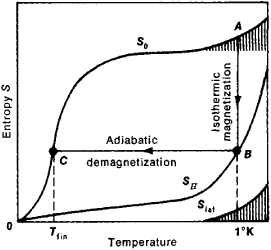
\includegraphics[width=1.5in]{src/gsed_0001_0015_0_img3696.png}
    \caption{Adiabatic demagnetization.}%
\end{marginfigure}%
\[ F = \rec{\beta}\Phi\pare{\beta H}, \]
and consequently
\[ S = k\+_B_\beta^2 \+D{\beta}DF = k\+_B_\brac{-\Phi\pare{\beta H} + \beta H\Phi'\pare{\beta H}}. \]
Therefore, $H/T$ is approximately constant.
\begin{termdef}{Adiabatic Demagnetization}
    In an adiabatic process on a system whose specific heat is dominated by the spin ststem, slowly lowering $H$ lowers $T$ as well.
\end{termdef}
At very low temperature, zero-field entropy prevents lowering the temperature further by this process.

% subsection adiabatic_demagnetization (end)

\subsection{Transition Metal Ions} % (fold)
\label{sub:transition_metal_ions}

\subsubsection{Crystal Field Theory} % (fold)
\label{ssub:crystal_field_theory}

\begin{margindef}[-3em]{CFT}
    Crystal Field Theory.
\end{margindef}
The $d$-electrons in transition metal ions experience inhomogeneous electric field produced by neighboring ions, i.e. the \gloss{crystal field}, which split the energy levels.\begin{margindef}[3em]{CFSE}
    Crystal Field Stablization Energy.
\end{margindef}
\begin{termdef}{Crystal Field Stablization Energy}
    The crystal field stablization energy is the energy of electron configuration in the ligand field minus the one in the isotropic field.
\end{termdef}
\begin{termdef}[1em]{Strong-Field Ligands}
    Strong-field ligands are those that create a large splitting $\Delta$ of the $d$-orbitals.
\end{termdef}
\begin{termdef}{High-Spin}
    $d$-electrons are put into each of the five $d$-orbitals before any spin pairing occurs.
\end{termdef}
\ce{CN^-} and \ce{CO} are strong-field ligands, which favors high-spin states.\begin{margindef}[-3em]{HS}
    High-Spin.
\end{margindef}
\begin{termdef}[2em]{Weak-Field Ligands}
    Weak-field ligands are those that create a small splitting $\Delta$ of the $d$-orbitals.
\end{termdef}
\begin{termdef}[-1em]{Low-Spin}
    $d$-electrons are paired before put into each of the five $d$-orbitals.
\end{termdef}
\ce{I^-} and \ce{Br^-} are weak-field ligands, which favors low-spin states.\begin{margindef}[-4em]{LS}
    Low-Spin.
\end{margindef}
\begin{termdef}{Quenching of Angular Momentum}
    $\expc{L_z} \approx 0$ along any axis in the presence of crystal field.
\end{termdef}
%\begin{margindef}{Ligand}\RaggedRight
%    An ion or molecule attached to a metal atom by coordinate bonding.
%\end{margindef}
\begin{finaleq}{Octaheadral Field Splitting}
    \centerline{$\Delta\+_o_ = \SI{10}{\Dq},$}
\end{finaleq}
where \gloss[-\baselineskip]{Dq} stands for \textit{differential of quanta}.
\begin{finaleq}{Tetrahedral Field Splitting}
    \centerline{$\displaystyle \Delta\+_t_ = \frac{4}{9}\Delta\+_o_,$}
\end{finaleq}
\begin{finalbox}[label=myref]{Crystal Field Splitting of Various Geometries}
\begin{tikzpicture}[yscale=0.25,xscale=1.13]
    \draw (0,0) -- (0.16,0) (0.21,0) -- (0.37,0) (0.42,0) -- (0.58,0) (0.63,0) -- (0.79,0) (0.84,0) -- (1,0);
    % Oct Field
    \draw[dashed] (1,0) -- (2.3,6);
    \draw (2.3,6) -- (2.8,6) node[midway,above] {\footnotesize$\mathrm{d}_{x^2-y^2}$};
    \draw (2.9,6) -- (3.4,6) node[midway,above] {\footnotesize$\mathrm{d}_{x^2}$};
    \draw[draw=none] (2.3,6) -- (3.4,6) node[midway,below] {\footnotesize$\mathrm{e}\+_g_$};
    \draw[dashed] (1,0) -- (2,-4);
    \draw (2,-4) -- (2.5,-4) node[midway,below] {\footnotesize$\mathrm{d}_{xy}$};
    \draw (2.6,-4) -- (3.1,-4) node[midway,below] {\footnotesize$\mathrm{d}_{yz}$} node[midway,above] {\footnotesize$\mathrm{t}\+_2g_$};
    \draw (3.2,-4) -- (3.7,-4) node[midway,below] {\footnotesize$\mathrm{d}_{xz}$};
    % Levels
    \draw (1.9,6) node[anchor=east] {\footnotesize$\SI{6}{\Dq}$};
    \draw (1.9,-4) node[anchor=east] {\footnotesize$\SI{-4}{\Dq}$};
    % Sp Field
    \draw[dashed] (3.7,-4) -- (4.7, -5.1);
    \draw (4.7,-5.1) -- (5.2,-5.1) node[midway,below] {\footnotesize$\mathrm{d}_{yz}$};
    \draw (5.3,-5.1) -- (5.8,-5.1) node[midway,below] {\footnotesize$\mathrm{d}_{xz}$};
    \draw[dashed] (3.7,-4) -- (5.0, 2.3);
    \draw (5.0,2.3) -- (5.5,2.3) node[midway,below] {\footnotesize$\mathrm{d}_{xy}$};
    \draw[dashed] (3.4,6) -- (5.0, -4.3);
    \draw (5.0,-4.3) -- (5.5,-4.3) node[midway,above] {\footnotesize$\mathrm{d}_{x^2}$};
    \draw[dashed] (3.4,6) -- (5.0, 12.3);
    \draw (5.0,12.3) -- (5.5,12.3) node[midway,below] {\footnotesize$\mathrm{d}_{x^2-y^2}$};
    % Levels
    \draw (5.9,-5.1) node[anchor=north west] {\footnotesize$\SI{-0.51}{\Dq}$};
    \draw (5.9,-4.3) node[anchor=south west] {\footnotesize$\SI{-4.3}{\Dq}$};
    \draw (5.9,2.3) node[anchor=west] {\footnotesize$\SI{2.3}{\Dq}$};
    \draw (5.9,12.3) node[anchor=west] {\footnotesize$\SI{12.3}{\Dq}$};
    % Tet Field
    \draw[dashed] (0,0) -- (-1,1.78);
    \draw (-1,1.78) -- (-1.5,1.78) node[midway,above] {\footnotesize$\mathrm{d}_{xz}$};
    \draw (-1.6,1.78) -- (-2.1,1.78) node[midway,above] {\footnotesize$\mathrm{d}_{yz}$} node[midway,below] {\footnotesize$\mathrm{t}_2$};
    \draw (-2.2,1.78) -- (-2.7,1.78) node[midway,above] {\footnotesize$\mathrm{d}_{xy}$};
    \draw[dashed] (0,0) -- (-1.3,-2.67);
    \draw (-1.3,-2.67) -- (-1.8,-2.67) node[midway,below] {\footnotesize$\mathrm{d}_{x^2}$};
    \draw (-1.9,-2.67) -- (-2.4,-2.67) node[midway,below] {\footnotesize$\mathrm{d}_{x^2-y^2}$};
    \draw[draw=none] (-1.3,-2.67) -- (-2.4,-2.67) node[midway,above] {\footnotesize$\mathrm{e}$};
    % Levels
    \draw (-2.8,1.78) node[anchor=east] {\footnotesize$\SI{1.78}{\Dq}$};
    \draw (-2.8,-2.67) node[anchor=east] {\footnotesize$\SI{-2.67}{\Dq}$};
    % Names
    \draw[draw=none] (-1,-7) -- (-2.7,-7) node[midway,below] {\bfseries Tetrahedral};
    \draw[draw=none] (-1,-9) -- (-2.7,-9) node[midway,below] {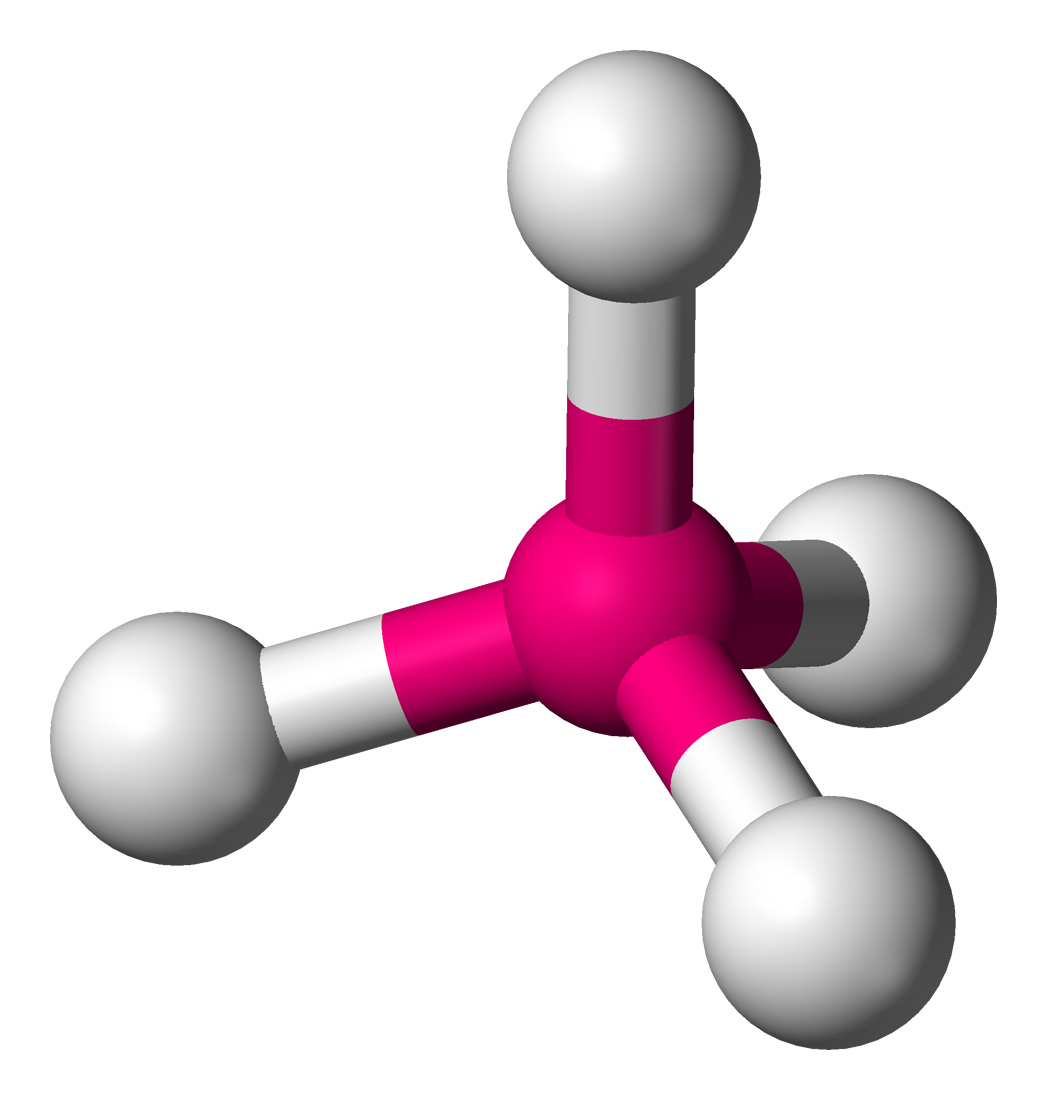
\includegraphics[width=3cm]{src/Tetrahedral-3D-balls.png}};
    \draw[draw=none] (2,-7) -- (3.7,-7) node[midway,below] {\bfseries Octahedral};
    \draw[draw=none] (2,-9) -- (3.7,-9) node[midway,below] {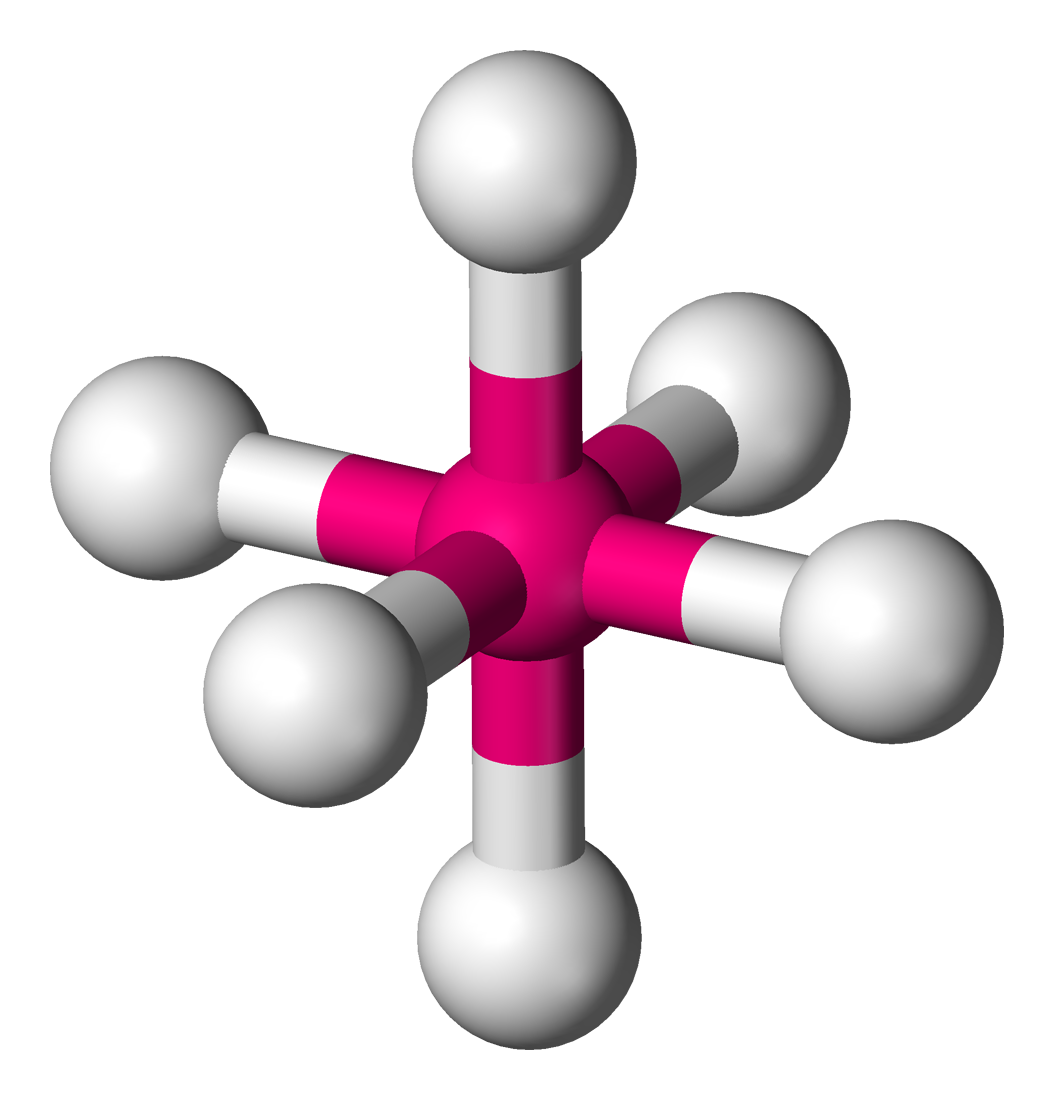
\includegraphics[width=3cm]{src/Octahedral-3D-balls.png}};
    \draw[draw=none] (4.7,-7) -- (5.8,-7) node[midway,below] {\bfseries Square Planar};
    \draw[draw=none] (4.7,-9) -- (5.8,-9) node[midway,below] {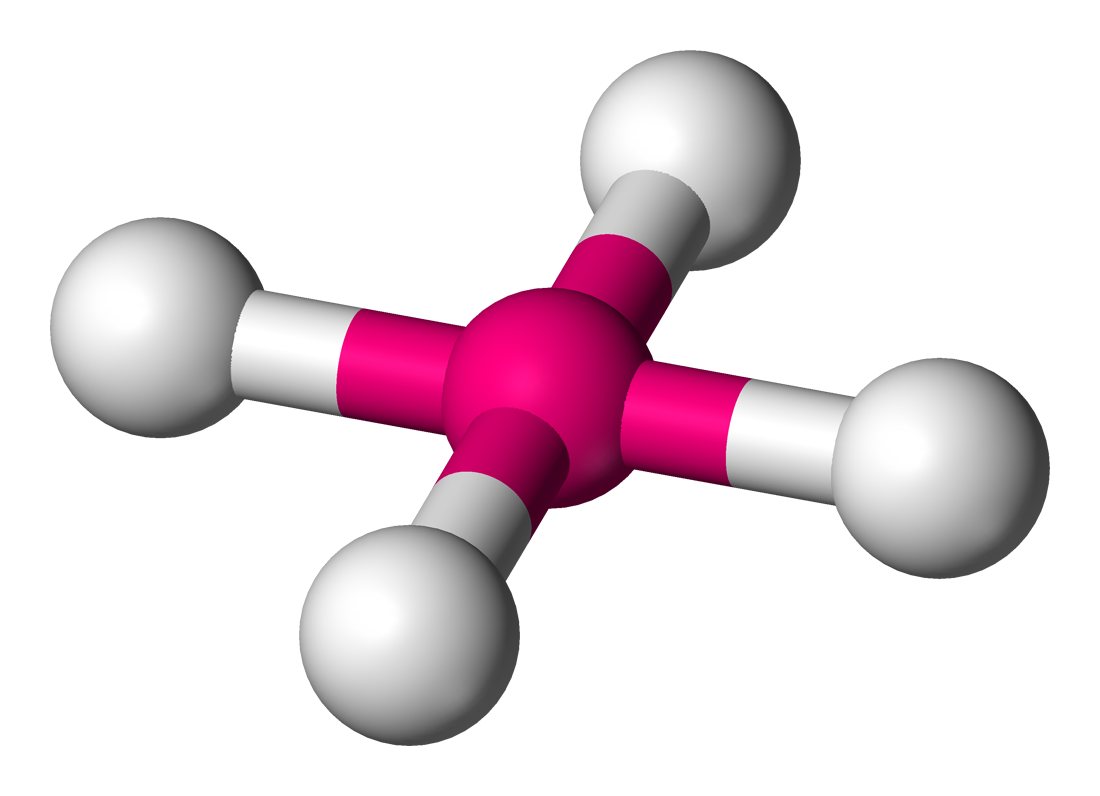
\includegraphics[width=3cm]{src/Square-planar-3D-balls.png}};
\end{tikzpicture}
\end{finalbox}
Due to the quenching of orbital angular momentum, the magnetic moment of each ion should be calculated as if $\+vL = 0$, i.e.
\[ \mu = \sqrt{n\pare{n+2}}\mu\+_B_, \]
where $n$ is the number of unpaird electrons.\marginnote{
\begin{tikzpicture}
    \elementcell{}{Cobalt}{CoCell}{Co}{58.9}{27}{$\mathrm{3d^74s^2}$};
\end{tikzpicture}
}
\begin{sample}
    \begin{example}
        In $\ce{Co(H2O)6^2+}$, the high-spin octahedral configuration is taken, and thus there are $3$ unpaired electrons, giving
        \[ \mu = \sqrt{3\times 5} = 3.87\mu\+_B_. \]
        The experimental data is $4.8\mu\+_B_$ and the error probably comes from the imperfect quenching of $\+vL$.
    \end{example}
\end{sample}
\vspace{-\baselineskip}
\begin{termdef}{Jahn-Teller Effect}
    Any non-linear molecule with a spatially degenerate electronic ground state will undergo a geometrical distortion that removes that degeneracy.
\end{termdef}
Complexes \begin{margindef}{SCO}
    Spin Crossover.
\end{margindef} of $\mathrm{d}^6$ ions show tendency to adopt the LS state at relatively weaker ligand fields than $\mathrm{d}^4$ and $\mathrm{d}^5$ complexes.

\paragraph{Manganese Compounds} % (fold)
\label{par:manganese_compounds}

\marginnote{
\begin{tikzpicture}
    \elementcell{}{\scriptsize Manganese}{MnCell}{Mn}{54.9}{25}{$\mathrm{3d^54s^2}$};
\end{tikzpicture}
}%
Almost all \ce{Mn(III)} complexes are known to be of HS ($S=2$). A slight decrease of the transition temperature of SCO is observed in \ce{[Mn(pyrol)3tren]} as well as in other complexes.
\par
Hysteresis loop in the $\chi$-$T$ curve may occur in complexes like \ce{Rb^I Mn^{II} [Fe^{III}(CN)6]} as well as FM ordering at \SI{12}{\kelvin} and below, due to temperature dependent electron transfer converting the complex from one spin state to another.

% paragraph manganese_compounds (end)

% subsubsection crystal_field_theory (end)

% subsection transition_metal_ions (end)

\subsection{Electron Interactions and Magnetic Structure} % (fold)
\label{sub:electron_interactions_and_magnetic_structure}

\subsubsection{Various Kinds of Exchange} % (fold)
\label{ssub:various_kinds_of_exchange}

In \gloss{Heitler-London approximation}, the symmetry and anti-symmetry spatial wave function is given by
\[ \begin{cases}
    \displaystyle \psi\+_S_\pare{\+vr_1,\+vr_2} = \rec{\sqrt{2}} \brac{\phi_\alpha\pare{\+vr_1}\phi_\beta\pare{\+vr_2} + \phi_\beta\pare{\+vr_1}\phi_\alpha\pare{\+vr_2}}, \\
\displaystyle \psi\+_A_\pare{\+vr_1,\+vr_2} = \rec{\sqrt{2}} \brac{\phi_\alpha\pare{\+vr_1}\phi_\beta\pare{\+vr_2} - \phi_\beta\pare{\+vr_1}\phi_\alpha\pare{\+vr_2}},
\end{cases} \]
where $\phi_1$ and $\phi_2$ are atomic orbits, from which the Coulomb energy difference could be calculated and shown to be proportional to $-\+vS_1\cdot \+vS_2$ with proper zero of energy.
\begin{termdef}{Direct Exchange}
    Direct exchange arises from the direct Coulomb interaction and the interchange symmetry.
\end{termdef}
Direct exchange is formulated by the \gloss{Heisenberg Hamiltonian}
\[ H^{\mathrm{spin}} = -\sum J_{ij} \+vS_i \cdot \+vS_j, \]
where $J_{ij}$ has to do with the exchange integral.
\begin{remark}
    For electrons on the same atom, $J_{ij}$ is usually positive, which stablizes the triplet state. However, electrons on different atoms may favor bonding in order to reduce energy, hence the singlet state and negative $J_{ij}$.
\end{remark}
\begin{termdef}{Superexchange}
    Superexchange is mediated by shared nonmagnetic neighbors.
\end{termdef}
Superexchange may occur when there are nonmagnetic ions between magnetic ones, for example in \ce{MnO}, where the antiferromagnetic configuration allows the electron be delocalized.
\par
The superexchange has $J \sim -t^2/U$ in second-order perturbation theory, where $t$ is the \gloss[-2\baselineskip]{hopping integral} and $U$ is the Coulomb energy, while $\Delta E \propto -t^4 \pare{\+vS_1\cdot \+vS_2}^2/U^3$ in fourth-order, known as \gloss[-2\baselineskip]{biquadratic exchange}.
\begin{termdef}{Indirect Exchange, RKKY Interaction}
    Indirect exchange is caused by $f$-electrons coupling with conduction electrons.
\end{termdef}
Indirect exchange can be seen in rare earth metals, where a localized magnetic moment spin-polarizes the conduction electrons and this polarization couples to a neighbouring localized magnetic moment a distance $r$ away. The coupling takes the form
\[ J\+_RKKY_\pare{r} \propto \frac{\cos \pare{2k\+_F_r}}{r^3}. \]\begin{marginfigure}
    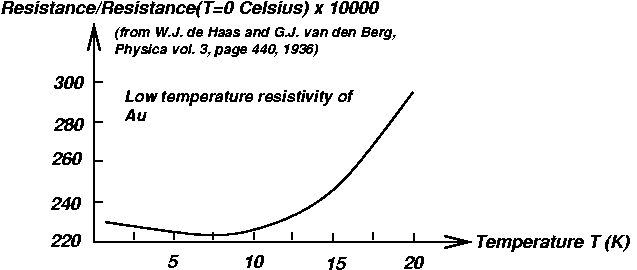
\includegraphics[width=2.10in]{src/Classickondo.png}
    \caption{Kondo effect.}
\end{marginfigure}

% subsubsection various_kinds_of_exchange (end)

\subsubsection{Kondo Effect} % (fold)
\label{ssub:kondo_effect}

Scattering of conduction electrons by magnetic ions in alloys at low temperatures may lead to increasing resistance with decreasing $T$,
\[ \rho = aT^5 + c\rho_0 - c\rho_1 \ln T, \]
and hence the Kondo effect.
\begin{termdef}{Kondo Effect}
    Resistance in alloys may increase with decreasing temperature and displays a minimal.
\end{termdef}

% subsubsection kondo_effect (end)

\subsubsection{Itinerant Exchange} % (fold)
\label{ssub:itinerant_exchange}

With spin polarized Hatree-Fock approximation
\[ E_{\uparrow/\downarrow} = N_{\uparrow/\downarrow}\brac{\frac{3}{5}\pare{k_{\uparrow/\downarrow} a_0}^2 - \frac{3}{2\pi}\pare{k_{\uparrow/\downarrow} a_0}}\cdot \frac{e^2}{2a_0}, \]
it could be found that a difference in $N_{\uparrow}$ and $N_{\downarrow}$ may lower the total energy if $k\+_F_$ is small enough, which induces magnetism.
\begin{termdef}{Itinerant Exchange}
    Itinerant exchange arises from conduction electrons themselves.
\end{termdef}
The above analysis in inaccurate and fragile, and thus itinerant exchange should be combined with specific features of the band structure and/or the kinds of atomic considerations leading to Hund's rules.

% subsubsection itinerant_exchange (end)

\subsubsection{Double Exchange} % (fold)
\label{ssub:double_exchange}

\begin{termdef}{Double Exchange}
    Itinerant exchange arises from conduction electrons themselves.
\end{termdef}

Double exchange arises between ions in different oxidation states. For example in \ce{Mn3+-O-Mn4+}, the electron may hop from one \ce{Mn} ion to another, reducing the overall kinetic energy and is easier if electrons in the $\mathrm{t_{2g}}$ orbits is aligned with those in the $\mathrm{e_{g}} orbits$, i.e. in a ferromagnetic configuration. 

% subsubsection double_exchange (end)

\subsubsection{Anisotropic Exchange Interaction} % (fold)
\label{ssub:anisotropic_exchange_interaction}

\begin{termdef}{Anisotropic Exchange Interaction, Dzyaloshinsky-Moriya Interaction}
    Spin-orbit interaction between the excited state of one ion and the ground state of the other ion.
\end{termdef}
The Hamiltonian is \begin{margindef}[2\baselineskip]{DMI}
    Dzyaloshinsky-Moriya Interaction.
\end{margindef}
\[ \hat{\+cH}\+_DM_ = \+vD\cdot \+vS_1 \times \+vS_2, \]
where $\+vD$ vanishes when the crystal field has an inversion symmetry with respect to the center beteen the two magnetic ions.
\par
This interaction tries to force $\+vS_1$ and $\+vS_2$ to be right angles in a plane perpendicular to the vector $\+vD$. Its effect is to cant the spins by a small angle, whih occurs commonly in antiferromagnets and result in a small ferromagnetic component perpendicular to the spin-axis of the antiferromagnet, known as \gloss{weak ferromagnetism}.

% subsubsection anisotropic_exchange_interaction (end)

% subsection electron_interactions_and_magnetic_structure (end)

\subsection{Magnetically Ordered Systems} % (fold)
\label{sub:magnetically_ordered_systems}

A system is \gloss{magnetically ordered} if invididual magnetic ions have nonvanishing average vector moments below a critical temperature $T_c$. In such systems, the \gloss[\baselineskip]{spin density}
\[ s_z\pare{\+vr} = \half \brac{n_{\uparrow}\pare{\+vr} - n_{\downarrow}\pare{\+vr}} \]
does not vanish locally.
\begin{experiment*}[NMR]
    Resonance is observed even without applied field in magnetically ordered systems.
\end{experiment*}
Magnetic ordering vanishes above the \gloss{critical temperature} $T_c$.
\begin{termdef}[\baselineskip]{Curie Temperature}
    The Curie temperature is the critical temperature in ferromegnets and ferrimagnets.
\end{termdef}%
\begin{termdef}[\baselineskip]{N\'eel Temperature}
    The N\'eel temperature is the critical temperature in antiferromagnets.
\end{termdef}%
The magnetization (sponetaneous magnetization in ferromagnets and ferrimagnets, and sublattice magnetization in antiferromagnets) is well described by
\begin{finaleq}{The Power Law of Magnetization}
    \centerline{$M\pare{T} \sim \pare{T_c - T}^\beta,$}
    for $T$ near $T_c$.
\end{finaleq}
where $\beta$ is typically between $0.33$ and $0.37$.
\par
Above the Curie temperature, in ferromagnets,
\[ \inlinefinaleq{\chi\pare{T} \sim \pare{T-T_c}^{-\gamma},} \]
where $\gamma$ is typically between $1.3$ and $1.4$. At the Curie temperature,
\[ \inlinefinaleq{M \propto H^{1/\delta}.} \]
\par%
There is also a singularity in zero-field specific heat as
\[ c\pare{T} \sim \pare{T-T_c}^{-\alpha}, \]
where $\alpha$ is typically $0.1$ or less.
\par
Near $T_c$, the magnetic equation of state has the form
\[ \frac{H}{\abs{T_c - T}^{\beta+\gamma}} = f_\pm \pare{\frac{M}{\abs{T_c-T}^{\beta}}},\quad T \gtrless T_c, \]
which is known as the \gloss{scaling equation of state}. The relation $\alpha + 2\beta + \gamma = 2$ fits the data well.
\begin{termdef}[\baselineskip]{Goldstone Bosons}
    Long-wavelength excitations produced by the small energy cost when breaking a continuous global symmetry.
\end{termdef}

\subsubsection{Landau Theory} % (fold)
\label{ssub:landau_theory}

The free energy is written as
\[ F\pare{M} = F_0 + a\pare{T} M^2 + bM^4 \]
where $b > 0$. Minimizing yields
\[ M = 0,\quad \text{or}\quad M = \pm \sqrt{\frac{a_0\pare{T_c - T}}{2b}}, \]
where the non-zero solutions occur only when $T<T_c$, and the $M=0$ solution is unstable for $T<T_c$.

% subsubsection laudau_theory (end)

\subsubsection{Heisenberg Model} % (fold)
\label{ssub:heisenberg_model}

The Heisenberg model is described by the Heisenberg Hamiltonian.
\begin{finaleq}{The Heisenberg Hamiltonian}
    \centerline{$\displaystyle \+sH = -\half \sum_{\+vR,\+vR'} J\pare{\+vR - \+vR'} \+vS\pare{\+vR}\cdot \+vS\pare{\+vR'} - g\mu\+_B_H \sum_{\+vR}\+vS_z\pare{\+vR}.$}\vspace{.5em}
    where $H$ is the local field and $J\pare{\+vR - \+vR'} = J\pare{\+vR' - \+vR} \ge 0$.
\end{finaleq}

% subsubsection heisenberg_model (end)

\subsubsection{Continuum Approximation} % (fold)
\label{ssub:continuum_approximation}

Assuming that $J_{ij}$ in the Heisenberg model is nonzero only for $i = j\pm 1$, and that the angle between the nearest neighbour spins $\phi_{ij}$ is small,
\begin{align*}
    E &= -JS^2 \sum_{\expc{ij}} \cos \phi_{ij} + \frac{JS^2}{2}\sum_{\expc{ij}}\phi_{ij}^2 = \frac{JS^2}{2} \sum_{\expc{ij}} \brac{\pare{\+vr_{ij}\cdot \grad}\+um}^2 \\
    &= A \int_V \brac{\pare{\grad m_x}^2 + \pare{\grad m_y}^2 + \pare{\grad m_z}^2}\,\rd{^3r},
\end{align*}
where $\expc{ij}$ denotes a sum over nearest neighbours only and $A = 2JS^2 z/a$.

% subsubsection continuum_approximation (end)

\subsubsection{High Temperature Susceptibility} % (fold)
\label{ssub:high_temperature_susceptibility}

With the energy levels given by the $\+sH$ above, we have\begin{margintips}
    Differentiate on $H$ in $e^{-\beta F} = Z$ and notice that $\expc{\+vS_z}_{H=0} = 0$ at high $T$.
\end{margintips}
\[ \chi\pare{T} = \rec{V}\frac{\pare{g\mu\+_B_}^2}{k\+_B_T}\expc{\brac{\sum_{\+vR} \+vS_z\pare{\+vR}}^2}_{H=0}, \]
where the mean value is of the Boltzmann distribution $n \propto e^{-\beta E_n}$. It can be proved that
\[ \expc{\+vS_z\pare{\+vR}\+vS_z\pare{\+vR'}}_{H=0} = \frac{S\pare{S+1}}{3}\brac{\delta_{\+vR,\+vR'} + \frac{S\pare{S+1}}{3}\beta J\pare{\+vR - \+vR'} + O\pare{\beta_J}^2}. \]
Therefore,
\begin{finaleq}{$\chi$ at High $T$}
    For large $T$, with $\displaystyle \theta = \frac{S\pare{S+1}}{3}\frac{J_0}{k\+_B_}$ and $\displaystyle J_0 = \sum_{\+vR} J\pare{\+vR}$,
    \[ \chi\pare{T} = \frac{N}{V}\frac{\pare{g\mu\+_B_}^2}{3k\+_B_T}S\pare{S+1}\brac{1+\frac{\theta}{T} + O\pare{\frac{\theta}{T}}^2}. \]
\end{finaleq}
This offers a way to distinguish between ferrimagnetism and ferrimagnetism/antiferromagnetism by checking whether $\theta>0$ or not.

% subsubsection high_temperature_susceptibility (end)

\subsubsection{Ising Model} % (fold)
\label{ssub:ising_model}

The Ising model is a simplification of the Heisenberg Model.
\begin{finaleq}{The Ising Hamiltonian}
    \centerline{$\displaystyle \+sH = -\half \sum_{\+vR,\+vR'}J\pare{\+vR - \+vR'}\+vS_z\pare{\+vR}\+vS_z\pare{\+vR'} - g\mu\+_B_H \sum_{\+vR}\+vS_z\pare{\+vR}.$}
\end{finaleq}
\begin{remark}
    The Ising model is of order parameter $D=1$ while the Heisenberg modelis of $D=3$.
\end{remark}

\paragraph{The one-dimensional Ising model} % (fold)
\label{par:the_one_dimensional_ising_model}

The Hamiltonian is
\[ \hat{\+cH} = -2J\sum_{i=1}^N S_i^z S_{i+1}^z, \]
which has the ground state energy $-NJ/2$ where all spins are aligned. Adding one defect yields an extra energy $E=J$ and an entrypy gain $S = k\+_B_\ln N$. When $N$ is large enough, the defect lowers $F = E - TS$ and is therefore more favorable as long as $T>0$. The critical temperature in this case is $T_c = 0$.

% paragraph the_one_dimensional_ising_model (end)

\paragraph{The two-dimensional Ising model} % (fold)
\label{par:the_two_dimensional_ising_model}

The two-dimensional model has a non-zero critical temperature because the entropy gain scales with the perieter sieze of the defect, and therefore the energy and entropy have a fair fight with each other.

% paragraph the_two_dimensional_ising_model (end)

% subsubsection ising_model (end)

\subsubsection{Mean Field Theory} % (fold)
\label{ssub:mean_field_theory}

\begin{margindef}{MFT}
    Mean Field Theory.
\end{margindef}
Approximating $\+vS\pare{\+vR}$ in the Heisenberg Hamiltonian with $\displaystyle \expc{\+vS\pare{\+vR}} = \frac{V}{N}\frac{\+vM}{g\mu\+_B_}$, we obtain the \gloss[\baselineskip]{Weiss model} for a single spin $\+vS\pare{\+vR}$ that
\[ \Delta \+sH = -g\mu\+_B_\+vS\pare{\+vR}\cdot \+vH\+_eff_, \]
where\begin{marginwarns}
    MFT fails to predict the Bloch $T^{3/2}$ law.
\end{marginwarns}
\[ \+vH\+_eff_ = \+vH + \lambda \+vM,\quad \lambda = \frac{V}{N}\frac{J_0}{\pare{g\mu\+_B_}^2},\quad J_0 = \sum_{\+vR}J\pare{\+vR}. \]
We learn from equation \eqref{eq:MomentsInTAndH} that $M$ depends on $H$ and $T$ only through $H/T$,
\[ M = M_0 \pare{\frac{H\+_eff_}{T}} = M_0\pare{\frac{\lambda M}{T}}, \]
therefore the following two equations\begin{marginwarns}
    MFT fails to predict the power law of $\chi$ near $T_c$.
\end{marginwarns}
\[ M\pare{T} = M_0\pare{x},\quad M\pare{T} = \frac{T}{\lambda} x \]
holds if spontaneous magnetization occurs, and consequently
\[ \chi_0 = \pare{\+DHD{M_0}}_{H=0} = \frac{M'_0\pare{T}}{T}, \]
whence a comparison with the explicit form of Curie's law, i.e. equation \eqref{eq:CuriesLaw} yields
\begin{finaleq}{$T_c$ of MFT}
    \centerline{$\displaystyle T_c = \frac{S\pare{S+1}}{3k\+_B_}J_0.$}
\end{finaleq}
The susceptibility is given by $\displaystyle \chi  = \+DHDM = \+D{H\+_eff_}D{M_0}\+DHD{H\+_eff_} = \chi_0\pare{1+\lambda \chi}$. Hence, applying the relation of $\lambda$ in $T_c$,
\begin{finaleq}{Curie-Weiss Law}
    \centerline{$\displaystyle \chi = \frac{\chi_0}{1-T_c/T} = \frac{C}{T-T_c}.$}
\end{finaleq}
Adding \begin{marginwarns}[-2\baselineskip]
    MFT ignores correlations and fluctuations which are important near $T_c$.
\end{marginwarns} a magnetic field shift the straight line to the right and therefore $M\neq 0$ for all temperatures. At $T = T_c$ we have $M \propto B^{1/3}$.
\par
Spin-orbit coupling may be ignored in transition metals thanks to quenching of angular momentum. In rare earth metals, however, the $g$ factor arising from spin-orbit coupling must be taken into account and the Curie temperature is written \marginnote{\inlinehardlink{\S 5.1.4, Blundell.}}
\[ T_c = \frac{z\pare{g_J - 1}^2J_0}{3k\+_B_}J\pare{J+1}, \]
where $z$ is the number of sites in the unit cell.

% subsubsection mean_field_theory (end)

% subsection magnetically_ordered_systems (end)

\subsection{Ferromagnetism} % (fold)
\label{sub:ferromagnetism}

In the ordered state of \gloss{spontaneous magnetization} occurs, individual localized moments add up to a net magnetization density, which is described as ferromagnetic.
\begin{termdef}[\baselineskip]{Ferromagnetic}
    A ferromagnetic compound has unpaired electron spins which are held in alignment.
    \begin{citemize}
        \item Strongly attracted to magnets.
    \end{citemize}
\end{termdef}%
\begin{marginfigure}%
\captionsetup{justification=raggedright, width=1.5in}
    \begin{tikzpicture}[xscale=0.5]%
        \draw(-1,0);
        \draw[-latex] (0,0) -- (0,1);
        \draw[-latex] (1,0) -- (1,1);
        \draw[-latex] (2,0) -- (2,1);
        \draw[-latex] (3,0) -- (3,1);
        \draw[-latex] (4,0) -- (4,1);
        \draw[-latex] (5,0) -- (5,1);
    \end{tikzpicture}%
    \caption{Ferromagnetism.}%
\end{marginfigure}%

%\subsubsection{The Weiss Model} % (fold)
%\label{ssub:the_weiss_model}

%The effective \gloss{molecular field} at site $i$ by
%\[ \+vB\+_mf_ = -\frac{2}{g\mu\+_B_} \sum_j J_{ij} \+vS_j. \]
%Therefore, with Zeeman effect any interaction with neighbour spins taken into account, the effective Hamiltonian on a single spin is
%\[ \hat{\+cH} = g\mu\+_B_ \sum_i \+vS_i \cdot \pare{\+vB + \+vB\+_mf_},\quad \text{where}\quad \+vB\+_mf_ = \lambda \+vM. \]
%To find a solution, we have to solve
%\[ \frac{M}{M\+_s_} = B\+_J_\pare{y},\quad y = \frac{g\+_J_\mu\+_B_ J\pare{B+\lambda M}}{k\+_B_T}. \]
%For high $T$, there is only one solution near $M = 0$. When $T<T_C$, there are three solutions, two of which near $M = M_S$ and are stable, leading to \gloss{spontaneous magnetization}.

% subsubsection the_weiss_model (end)

\subsubsection{Ground State of Ferromagnetism} % (fold)
\label{ssub:ground_state}

With each $\ket{S}_{\+vR}$ taking the maximal eigenvalue $S$ of $\+vS_z$, the Heisenberg Hamiltonian yields the minimal
\[ E = -\half S^2 \sum_{\+vR,\+vR'} J\pare{\+vR - \+vR'} - Ng\mu\+_B_HS. \]

% subsubsection ground_state (end)

\subsubsection{Spin Waves in Ferromagnets} % (fold)
\label{ssub:spin_waves}

With $\ket{\+vR}$ denoting the state which differs from the ground state by lowering $\+vS_z$ at site $\+vR$ to $S-1$,\begin{marginfigure}
    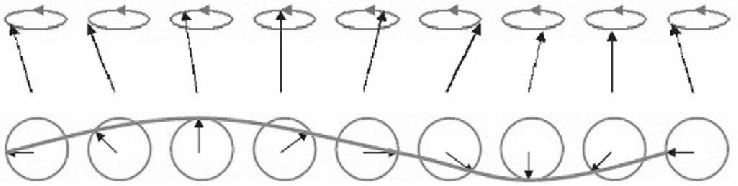
\includegraphics[width=1.5in]{src/A-spin-wave-on-a-spin-chain-Top-the-spins-viewed-in-perspective-Bottom-the-spins-gray.png}
    \caption{Spin wave.}
\end{marginfigure}%
\begin{equation}
    \label{eq:SpinWave}
    \ket{\+vk} = \rec{\sqrt{N}}\sum_{\+vR} e^{i\+vk\cdot \+vR}\ket{\+vR}
\end{equation}
is an eigenstate of $\+sH$ with excitation energy
\[ \+cE\pare{\+vk} = E_{\+vk} - E_0 = g\mu\+_B_H + 2S\sum_{\+vR} J\pare{\+vR}\sin^2\pare{\half \+vk\cdot \+vR} \]
and total spin $NS - 1$. With $\+vS_\perp = \+vS_x \+ux + \+vS_y \+uy$,
\[ \bra{\+vk}\+vS_\perp\pare{\+vR}\cdot \+vS_\perp\pare{\+vR'}\ket{\+vk} = \frac{2S}{N}\cos \brac{\+vk\cdot\pare{\+vR - \+vR'}}, \]
making $\ket{\+vk}$ wave-like.
\begin{termdef}{Spin Wave}
    Spin waves are periodic disturbances in spins from the ground state as in equation \eqref{eq:SpinWave}.
\end{termdef}
Retaining only the interation between nearest neighbors in the Heisenberg model,\begin{marginfigure}
    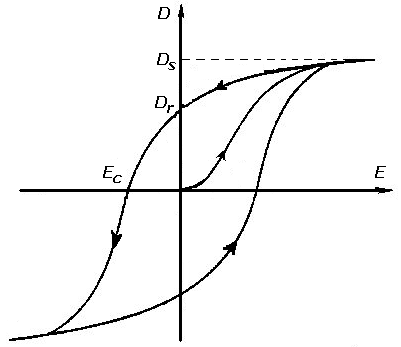
\includegraphics[width=1.5in]{src/Ehysteresis.png}
    \caption{Hysteresis loop.}
\end{marginfigure}
\begin{equation}
    \label{eq:NearestHeisenberg}
    U = -2J\sum_{p=1}^N \+vS_p\cdot \+vS_{p+1},
\end{equation}
we found $\+vS_p$ precessing as
\[ \+dtd{\+vS_p} = \frac{2J}{\hbar}\pare{\+vS_p \times \+vS_{p-1} + \+vS_p \times \+vS_{p+1}}, \]
and therefore
\[ \hbar\omega = 4JS\pare{1-\cos ka} \approx \pare{2JSa^2}k^2, \]
where the approximation holds for $ka \ll 1$, i.e. for long wavelengths.
\begin{finaleq}{Dispersion Relation of Spin Waves}
    \centerline{$h\omega = \pare{2JSa^2}k^2.$}
\end{finaleq}
Following the similar quantization steps as for phonons,\begin{margindef}{Magnon}
    A magnon is a quantized spin wave.
\end{margindef} we have
\[ E_{\+vk} = \pare{n_{\+vk} + \half}\hbar\omega_k \]
for magnons. Since $\displaystyle \sum n_k/NS$ is equal to $\Delta M/M\pare{0}$, we found
\begin{align*}
    M\pare{T} &= M\pare{0}\brac{1-\rec{NS}\sum_{\+vk}n\pare{\+vk}} = M\pare{0}\brac{1 - \frac{V}{NS}\int \frac{\rd{\+vk}}{\pare{2\pi}^3}}\rec{e^{\+cE\pare{\+vk}/k\+_B_T} - 1}\\
    &\approx M\pare{0}\brac{1-\frac{V}{NS}\pare{k\+_B_T}^{3/2}\int \frac{\rd{\+vq}}{\pare{2\pi^3}}\curb{\exp\brac{S\sum_{\+vR}J\pare{\+vR}\frac{\pare{\+vq\cdot \+vR}^2}{2}} - 1 }^{-1} },
\end{align*}
whence, in isotropic ferromagnets,
\begin{finaleq}{Bloch $T^{3/2}$ Law}
    \centerline{$\displaystyle 1 - \frac{M\pare{T}}{M\pare{0}} \propto T^{3/2},$}
    for $T \approx 0$.
\end{finaleq}
The energy is calculated to be $E\+_magnon_ \propto T^{5/2}$, giving a heat capacity proportional to $T^{3/2}$ at low temperatures.
\begin{figure}[ht]
    \centering
    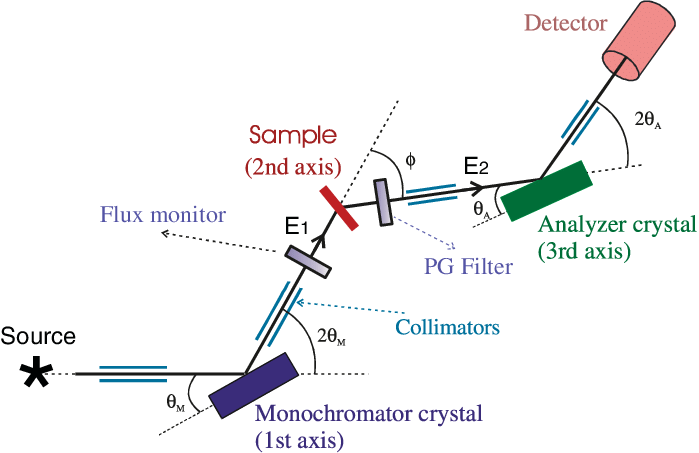
\includegraphics[width=8cm]{src/Schematic-drawing-of-the-triple-axis-spectrometer-The-monochromator-crystal-at-the-first.png}
    \caption{A neutron triple-axis spectrometer.}
    \label{fig:neutron_triple_axis_spectrometer}
\end{figure}
\begin{experiment*}[Neutron Magnetic Scattering]
    By conservation of crystal momentum and energy,
    \[ \+vk_n = \+vk'_n + \+vk + \+vG,\quad \frac{\hbar^2 k_n^2}{2M\+_n_} = \frac{\hbar^2 k'^2_n}{2M\+_n_} + \hbar\omega_{\+vk} \]
    holds for neutrons scattered by magnetic structures and creating of annihilating a magnon, whence dispersion relations of magnons can be determined.
    \par
    The measurement is done with a neutron triple-axis spectrometer as shown in \cref{fig:neutron_triple_axis_spectrometer}.
\end{experiment*}

The number of spin waves which are generated at finite temperature diverges for 1-D and 2-D Heisenberg models.
\begin{finaleq}{The Merlin-Wagner-Berenzinskii Theorem}
    In the isotropic 1-D and 2-D Heisenberg models, there can be no ferromagnetism at $T>0$.
\end{finaleq}
However, anisotropy may suppress the fluctuations and therefore ferromagnetism at finite temperature may exists.

% subsubsection spin_waves (end)

\subsubsection{Domains} % (fold)
\label{ssub:domains}

While short-range exchange interactions favours parallel spins, long-range dipole interactions favours antiparallel ones. Magnetized specimen is devided into \gloss{domains} whose magnetization vectors points in different directions.
\begin{termdef}{Hysteresis}
    Hysteresis is the phenomenon that stronger field is required to return a magnetized specimen to its unmagnetized state.
\end{termdef}
\begin{termdef}{Coercive Force}
    Coercive force is the field required to restore a zero magnetization.
\end{termdef}
\begin{termdef}{Soft Magnetic}
    Materials with low coercivity are called soft.
\end{termdef}
\begin{termdef}{Hard Magnetic}
    Materials with high coercivity are called hard.
\end{termdef}
\begin{termdef}[-2.5\baselineskip]{Anisotropy Energy}
    Anisotropy energy is the energy in a ferromagnetic crystal that directs the magnetization along directions easy magnetization.
\end{termdef}
For example, in hexagonal crystals (e.g. for Cobalt), \begin{marginfigure}[-2.5cm]%
\captionsetup{justification=raggedright, width=1.5in}
    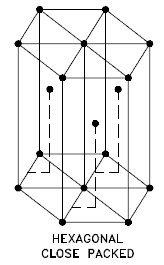
\includegraphics[width=1in]{src/Hexagonal-Close-packed-hcp-crystal-structure.png}
    \caption{Hexagonal Structure.}%
\end{marginfigure}%
the anisotropy energy is
\[ U_K = K'_1 \sin^2\theta + K'_2\sin^4 \theta, \]
which is a \gloss[3\baselineskip]{uniaxial anisotropy}. In cubic crystals (e.g. for Iron), however, it is
\[ U_K = K'_1\pare{\alpha_1^2 \alpha_2^2 + \alpha_2^2\alpha_3^2 + \alpha_3^2\alpha_1^2} + K_2\alpha_1^2\alpha_2^2\alpha_3^2, \]
where $\alpha_1$, $\alpha_2$ and $\alpha_3$ are direction cosines. Anisotropy energies are larger in lattices of low symmetry.
%\par
%An \begin{margindef}[-5\baselineskip]{Demagnetizing Field}
%    The $\+vH$ field generated by the magnetization in a magnet.
%\end{margindef} additional energy term is due to the demagnetizing energy associated with the sample shape and is referred to as \gloss[-\baselineskip]{shape anisotropy}. In thin films it is $\displaystyle \half \mu_0 M^2 \cos^2 \theta$.
\begin{termdef}[\baselineskip]{Bloch Wall}
    The Bloch wall is the transition layer between adjacent domains magnetized in opposite ($\SI{180}{\degree}$) directions.
\end{termdef}
\begin{termdef}{N\'eel Wall}
    The N\'eel wall is the transition layer between adjacent domains magnetized in perpendicular ($\SI{90}{\degree}$) directions.
\end{termdef}
The energy per unit area of the wall in the sum of the exchange energy and anisotropy energy,
\[ \sigma\+_w_ = \sigma\+_ex_ + \sigma\+_aniso_ = \frac{\pi^2JS^2}{Na^2} + KNa \xlongrightarrow{\mathrm{minimize}} \sigma\+_w_ \approx 2\pi\pare{\+/KJS^2/a/}^{\half},\ N \approx \pare{\+/\pi^2 JS^2/Ka^3/}^{\half}. \]
$N\approx 300$ for order of magnitude in iron.
\par
The domain structure originates from its ability to lower $\displaystyle \int B^2$, the magnetic energy. A \gloss[-8\baselineskip]{closure domain} structure may finally be formed an eliminates the dipole energy but introduces a number of domain walls.
\par
The length of a ferromagnetic changes slightly when it is magnetized. This effect is known as \gloss[3\baselineskip]{magnetostriction}. The crystal deforms because it can lower its anisotropy energy.
\begin{termdef}{Barkhausen Effect}
    The magnetization of a ferromagnet changes by a series of discontinuous steps due to domain boundary motion, so that very small steps are sometimes seen on the magnetization curves.
\end{termdef}
Therefore in low leve lacoustic emission also sometimes accompanies the magnetization process, a effect known as \gloss{magnetoacoustic emission}.
\begin{experiment*}[Kerr Microscopy]
    The polarization plane of a beam may rotation after reflection by a magnetic sample, known as the Kerr effect.
\end{experiment*}
\begin{experiment*}[Lorentz Microscopy]
    Electron beams are deflected by the Lorentz force due to the internal field.
\end{experiment*}
\begin{experiment*}[Magnetic Force Microscopy]
    The magnetized tip may bent the tiny cantilever it is attached to, which may be detected by the change in resonant frequency.
\end{experiment*}

% subsubsection domains (end)

\subsubsection{Small Magnetic Particles} % (fold)
\label{ssub:small_magnetic_particles}

In many ferromagnetic samples the lowest energy state at zero applied field is the demagnetized state, so that the overall magnetic moment is zero. For samples of small size, the surface energies may be significant and the critical and it may be energetically favorable to remove the domain walls and the sample is therefore a single magnetized domain. The critical size is given by $E\+_demagnetization_ = E\+_wall_$.

\paragraph{Stoner-Wohlfarth Model} % (fold)
\label{par:stoner_wohlfarth_model}

If the magnetic field $\+vH$ is applied at an angle $\theta$ to the easy axis of its uniaxial anisotropy and the magnetization of the particle lies at an angle of $\phi$ to the magnetic field direction, the energy density is
\[ E = K\sin^2\pare{\sin-\varphi} - \mu_0 HM_s \cos\phi. \]
The minimization of this energy yields the direction of the magnetization. Also, hysteresis loop may be obtained in this way.

% paragraph stoner_wohlfarth_model (end)

% subsubsection small_magnetic_particles (end)

% subsection ferromagnetism (end)

\subsection{Ferrimagnetism} % (fold)
\label{sub:ferrimagnetism}

\begin{termdef}[\baselineskip]{Ferrimagnetic}
    A ferrimagnetic compound has unpaired electrons which favors antiparallel alignment but failed to cancel their moments.
    \begin{citemize}
        \item Attracted to magnets.
    \end{citemize}
\end{termdef}%
\begin{marginfigure}%
\captionsetup{justification=raggedright, width=1.5in}
    \begin{tikzpicture}[xscale=0.5]%
        \draw(-1,0);
        \draw[-latex] (0,0) -- (0,1);
        \draw[latex-] (1,0) -- (1,.5);
        \draw[-latex] (2,0) -- (2,1);
        \draw[latex-] (3,0) -- (3,.5);
        \draw[-latex] (4,0) -- (4,1);
        \draw[latex-] (5,0) -- (5,.5);
    \end{tikzpicture}%
    \caption{Ferrimagnetism.}%
\end{marginfigure}%
\begin{margindef}[1cm]{Spinel Structures}\RaggedRight
    Spinel structures have the general formula \ce{AB2O4}.
    The normal/inverse spinel structures are shown in \cref{fig:SpinelStructures}.
\end{margindef}
\begin{figure}[ht]
    \centering
    \begin{subfigure}[t]{.3\textwidth}
        \centering
        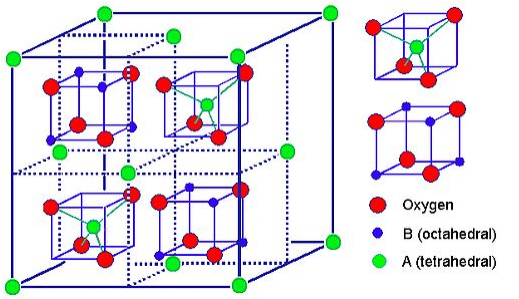
\includegraphics[height=1in]{src/spinel.png}
        \caption{Normal spinel structure. \ce{A^2+} ions occupy tetrahedral sites, while \ce{B^3+} ions occupy octaheadral sites.}
        \label{fig:NormalSpinelStructure}
    \end{subfigure}
    \begin{subfigure}[t]{.66\textwidth}
        \centering
        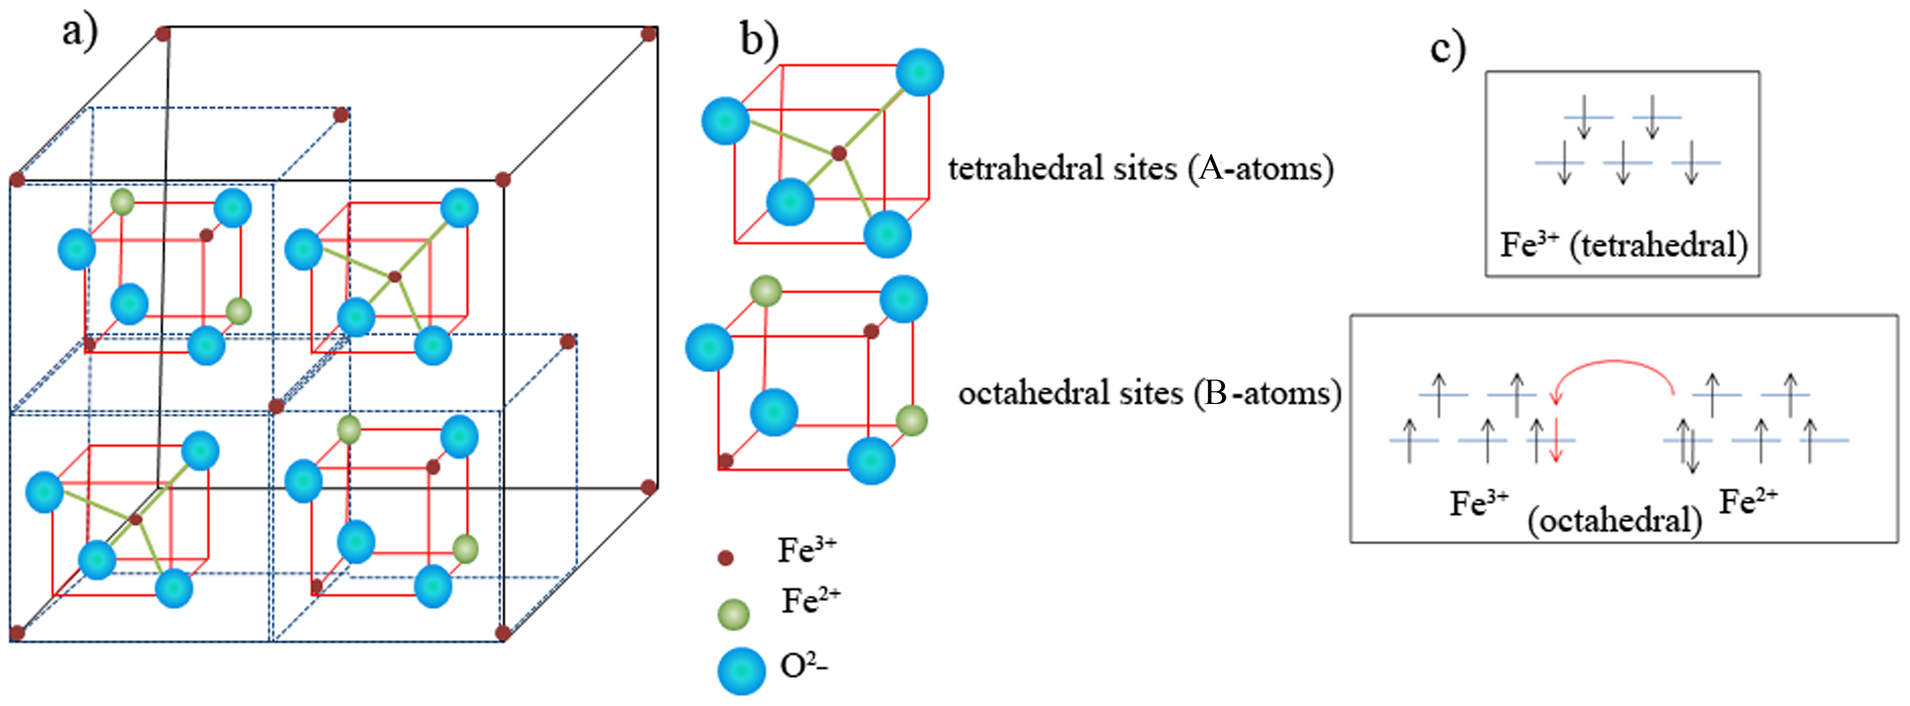
\includegraphics[height=1in]{src/inverse-spinel.png}
        \captionsetup{width=0.75\textwidth}
        \caption{Inverse spinel structure. \ce{A^2+} ions occupy half of the octaheadral sites, while \ce{B^3+} ions occupy another half of the octabheadral sites and tetrahedral sites.}
        \label{fig:InverseSpinelStructure}
    \end{subfigure}
    \caption{Spinel structures.}
    \label{fig:SpinelStructures}
\end{figure}
Ferrimagnetism can be seen in ferrites,\begin{margindef}{Ferrite}
    Ferrite has the formula \ce{MO\cdot Fe2O3}.
\end{margindef} which have the spinel structure shown in \cref{fig:SpinelStructures}. The exchange integrals $J_{AA}$, $J_{BB}$ and $J_{AB}$ are all negative and therefore favour antiparallel alignment of spins.
\par
Sometimes one sublattice can dominate the magnetization at low temperature but another dominates at higher temperature.
\begin{termdef}[5\baselineskip]{Compensation Temperature}
    The temperature at which the net magnetization in a ferrimagnet reduces to zero.
\end{termdef}
\gloss[2\baselineskip]{Garnets} belong to another family of ferrimagnets, which have the chemical formula \ce{R3Fe5O12}.

\subsubsection{Curie Temperature and Susceptibility of Ferrimagnets in MFT} % (fold)
\label{ssub:curie_temperature_and_susceptibility_of_ferrimagnets}

With $\+vB_A = -\mu \+vM_B$ and $\+vB_B = -\mu \+vM_A$ in the MFT for simplicity, we have via Curie's law the approximation
\[ M_A T = C_A\pare{B\+_applied_ - \mu M_B},\quad M_B T = C_B\pare{B\+_applied_ - \mu M_A}. \]
Solving for $M_A$ and $M_B$ and substituting them for $\displaystyle \chi = \frac{M_A+M_B}{B\+_applied_}$ we get
\begin{finaleq}{Susceptibility of Ferrimagnets}
    for $T>T_c$,
    \[ \chi = \frac{\pare{C_A+C_B}T - 2\mu C_AC_B}{T^2 - T_c^2}, \]
\end{finaleq}
where
\begin{finaleq}{Curie Temperature of Ferrimagnets}
    \centerline{$\displaystyle T_c = \mu\pare{C_AC_B}^{1/2}.$}
\end{finaleq}

% subsubsection curie_temperature_and_susceptibility_of_ferrimagnets (end)

% subsection ferrimagnetism (end)

\subsection{Antiferromagnetism} % (fold)
\label{sub:antiferromagnetism}

When individual local moments sum to zero, no spontaneous magnetization in present.%
\begin{termdef}{Antiferromagnetic}
    A antiferromagnetic compound has unpaired electrons held in alignment with an equal number of spins in each direction.
    \begin{citemize}
        \item Strongly repelled by a magnet.
    \end{citemize}
\end{termdef}%
\begin{marginfigure}%
\captionsetup{justification=raggedright, width=1.5in}
    \begin{tikzpicture}[xscale=0.5]%
        \draw(-1,0);
        \draw[-latex] (0,0) -- (0,1);
        \draw[latex-] (1,0) -- (1,1);
        \draw[-latex] (2,0) -- (2,1);
        \draw[latex-] (3,0) -- (3,1);
        \draw[-latex] (4,0) -- (4,1);
        \draw[latex-] (5,0) -- (5,1);
    \end{tikzpicture}%
    \caption{Antiferromagnetism.}%
\end{marginfigure}%
\begin{figure}[h]
    \centering
    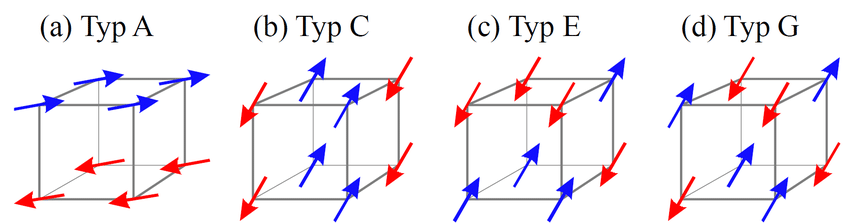
\includegraphics[width=.8\textwidth]{src/Several-possible-antiferromagnetic-order-patterns-for-a-simple-cubic-lattice-a.png}
    \caption{Antiferromagnetic order in simple cubic lattices.}
    \label{fig:antiferromagnetic_sc}
\end{figure}
There are various arrangement of anitiferromagnetism. Those of simple cubic lattices are shown in \cref{fig:antiferromagnetic_sc}.

\subsubsection{Ground State of Antiferromagnetism} % (fold)
\label{ssub:ground_state}

In the case where the spins resides on two lattices and each spin interacts only with those on the other sublattice,
\[ \+sH = \half \sum_{\+vR,\+vR'}\abs{J\pare{\+vR - \+vR'}}\+vS\pare{\+vR}\cdot \+vS\pare{\+vR'}. \]
The state where each sublattice is oppositely ferromagnetic is not an eigenstate. The energy of the ground state is estimated to be
\[ -\half S\pare{S+1} \sum_{\+vR,\+vR'}\abs{J\pare{\+vR - \+vR'}} \le E_0 \le -\half S^2 \sum_{\+vR,\+vR'}\abs{J\pare{\+vR-\+vR'}}. \]

% subsubsection ground_state (end)

\mathsubsubsection{NTSA}{N\'eel Tempera...}{N\'eel Temperature and Susceptibility of Antiferromagnets in MFT}{Neel Temperature and Susceptibility of Antiferromagnets in MFT} % (fold)
\label{ssub:neel_temperature_and_susceptibility_of_antiferromagnets}

Antiferromagnetism can be seen as a special case of ferrimagnetism where $C_A = C_B$ and therefore the N\'eel temperature and susceptibility are given by
\begin{finaleq}{N\'eel Temperature of Antiferromagnets}
    \centerline{$T\+_N_ = \mu C,$}
\end{finaleq}
and
\begin{finaleq}{Susceptibility of Antiferromagnets}
    \centerline{$\displaystyle \chi = \frac{2C}{T+\theta},$}
\end{finaleq}
respectively. $\theta$ is predicted to be $T\+_N_$ in the MFT, accurate only within a factor of four or so compared with experimental data.
\begin{termdef}{Staggered Magnetization}
    The difference of the magnetization $M_A - M_B$ on each lattice site.
\end{termdef}

% subsubsection neel_temperature_and_susceptibility_of_antiferromagnets (end)

\mathsubsubsection{SBNT}{Susceptibility...}{Susceptibility Below the N\'eel Temperature}{Susceptibility Below the Neel Temperature} % (fold)
\label{ssub:susceptibility_below_the_neel_temperature}

\begin{marginfigure}[\baselineskip]%
\captionsetup{justification=raggedright, width=1.5in}
    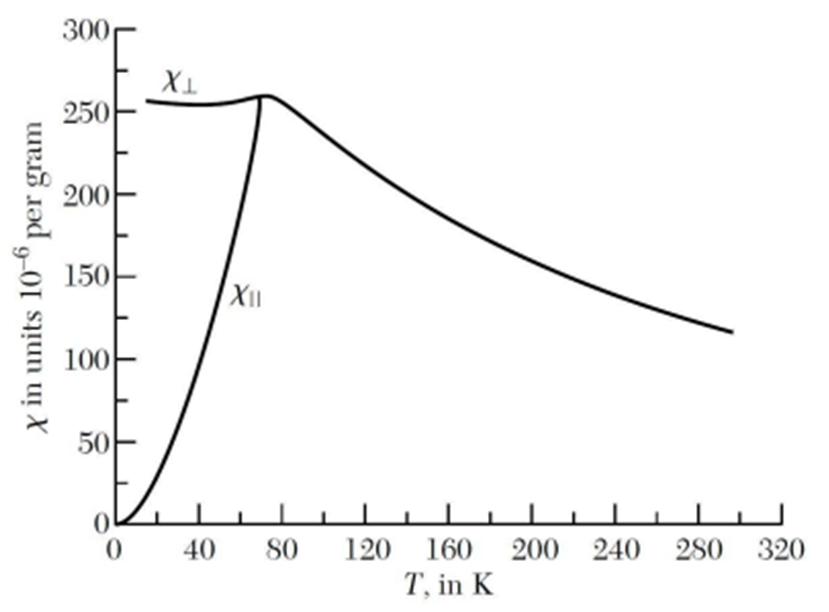
\includegraphics[width=1.5in]{src/Susceptibility-of-the-antiferromagnetic-MnF-2-17-The-kink-in-the-curve-happens-at.png}
    \caption{Temperature dependence of $\chi$ of an antiferromagnet.}%
\end{marginfigure}%
In antiferromagnets $\chi$ has a maximun a little above $T_c$, and drops on both sides of it. Anisotropy leads to different curves for $\chi_\perp$ and $\chi_\parallel$ below $T_c$.
\par
The energy density in the presence of an applied field is
\[ U = \mu \+vM_A\cdot \+vM_B - \+vB\+_applied_\cdot\pare{\+vM_A + \+vM_B}, \]
from which we deduce the susceptibility 
\[ \chi_\perp = \rec{\mu} \]
for $\+vB\+_applied_$ perpendicular to the spins, and
\[ \chi_\parallel\pare{T=0} = 0 \]
for $\+vB\+_applied_$ parallel to the spins at $\SI{0}{\kelvin}$.

% subsubsection susceptibility_below_the_neel_temperature (end)

\subsubsection{The Effect of a Strong Magnetic Field} % (fold)
\label{ssub:the_effect_of_a_strong_magnetic_field}

If the applied magnetic field is parallel to the sublattice magnetizations, the moments would not rotate until a critical temperature is reached.
\begin{termdef}{Spin-Flop Transition}
    Above the critical field the magnetic moments bends to the same side.
\end{termdef}
\begin{marginfigure}[-4\baselineskip]%
\captionsetup{justification=raggedright, width=1.5in}
    \begin{tikzpicture}[xscale=0.8]
        \draw[-latex] (0,-1) -- (0,1) node[midway,left] {$\+vB$};
        \fill (1,0) circle (0.1);
        \draw[-latex] (1,0) -- (1,1.5) node[midway, left] {$\+vM_+$};
        \draw[-latex] (1,0) -- (1,-1.5) node[midway, left] {$\+vM_-$};
        \draw[-latex] (2,-1) -- (2,1) node[midway,left] {$\+vB$};
        \fill (3,0) circle (0.1);
        \draw[-latex] (3,0) --++ (105:1.5) node[above] {$\+vM_+$};
        \draw[-latex] (3,0) --++ (75:1.5) node[above] {$\+vM_-$};
    \end{tikzpicture}
    \caption{Spin-flop transition.}%
\end{marginfigure}%
The energy is modelled by
\[ E = -2MB \cos\theta + AM^2 \cos 2\theta - \Delta \cos^2\theta, \]
where the last term is the anisotropy term. When $B$ is large enough, this energy may be lower than the antiferromagnetic $E = -AM^2 - \Delta$, leading to a spin-flop phase. When $\Delta$ is large enough, spin-flip transition may occur.
\begin{termdef}[\baselineskip]{Spin-Flip Transition}
    The magnetization of one sublattice suddenly reverses when $B$ reaches a critical value.
\end{termdef}

% subsubsection the_effect_of_a_strong_magnetic_field (end)

\subsubsection{Antiferromagnetic Magnons} % (fold)
\label{ssub:antiferromagnetic_magnons}

Retaining only nearest neighbor interations in one-dimensional anti-ferromagnets as in equation \eqref{eq:NearestHeisenberg} with $J<0$, we obtain the dispersion relation in this case
\[ \omega^2 = \omega\+_ex_^2\pare{1-\cos^2 ka}, \]
where $\omega\+_ex_ = 4\abs{J}S/\hbar$.
\begin{finaleq}{Dispersion Relation in Antiferromagnets}
    \centerline{$\omega = \omega\+_ex_\abs{\sin ka}.$}
\end{finaleq}

% subsubsection antiferromagnetic_magnons (end)

% subsection antiferromagnetism (end)

\subsection{Other Arrangements} % (fold)
\label{sub:other_arrangements}

\subsubsection{Helical Order} % (fold)
\label{ssub:helical_order}

In rare earth metals, atoms lie in layers. With the interaction between the layers modelled by a nearest-neighbour exchange constant $J_1$ and a next-nearest-neighbour exchange constant $J_2$, the energy of the system is
\[ E = -2NS^2\pare{J_1 \cos\theta + J_2 \cos 2\theta}, \]
where $N$ is the number of atoms in each plane. Minimizing the energy yields
\[ \cos\theta = -\frac{J_1}{4J_2}. \]
If $\abs{J_1} < \abs{4J_2}$ and $J_2 < 0$, the system exhibits helimagnetism. In other cases, it is either ferromagnetic or antiferromagnetic.
\begin{termdef}{Helimagnetism}
    Helimagnetism is a form of magnetic ordering where spins of neighbouring magnetic moments arrange themselves in a spiral or helical pattern.
\end{termdef}

% subsubsection helical_order (end)

\subsubsection{Spin Glasses} % (fold)
\label{ssub:spin_glasses}

\begin{termdef}{Spin Glass}
    A magnetic system with mixed random spins freezing below a temperature $T_f$, where a metastable fronzen state appears without the usual magnetic long-range ordering.
\end{termdef}
$T_f$ is called the \gloss{freezing temperature}.

% subsubsection spin_glasses (end)

\subsubsection{Nuclear Ordering} % (fold)
\label{ssub:nuclear_ordering}

The effect of nuclear spins is too way smaller than that of the electrons, observable only at extreme low temperatures.

% subsubsection nuclear_ordering (end)

% subsection other_arrangements (end)

\subsection{Measurement of Magnetic Order} % (fold)
\label{sub:measurement_of_magnetic_order}

\subsubsection{Magnetization and Magnetic Susceptibility} % (fold)
\label{ssub:magnetization_and_magnetic_susceptibility}

In \begin{margindef}[-4\baselineskip]{VSM}
    Vibrating Sample Magnetometer.
\end{margindef} an \gloss{extraction magnetometer}, the sample is placed at the center of a coil and then removed to a large distance, whence $\displaystyle \int V\,\rd{t}$ in the coil gives magnetic flex $\Phi$.
\par
A \gloss{vibrating sample magnetometer} vibrates a sample sinusoidally, which generates a electrical signal.
\par
In a \gloss{alternating gradient magnetometer}, the sample is mounted on a piezoelectric strip and subjected to a alternating field, which \begin{margindef}[\baselineskip]{Piezoelectricity}
    Electric charge accumulates under mechanical stress.
\end{margindef} deflects the strip and generates an electrical signal.
\par
In a \gloss[3\baselineskip]{torque magnetometer}, the sample is suspended on a torsion fibre, subjected to a field $\+vB$ which yields a torque $\+v\mu\times \+vB$.
\par
\gloss[3\baselineskip]{SQUID} (superconducting quantum interference device) may be used so that a persistent current is induced when a sample passes through.
\par
In the \gloss[2\baselineskip]{Gouy method} a long cylindrical sample is suspended between the pole pieces of a magnet, so that when the magnet is turned on and off, the apparent weight of the sample changes.
\par
In the \gloss{Faraday method}, a smaller sample is used and the force is produced by the gradient of $\+vB$.

% subsubsection magnetization_and_magnetic_susceptibility (end)

\subsubsection{Neutron Scattering} % (fold)
\label{ssub:neutron_scattering}

The neutron has magnetic moment coupling to electronic spins aside from being scattered by nuclei, which leads to peaks in elastic neutron scattering cross section varying with magnetic field and weaken or disappear with rising temperature.
\par
The amplitude of the magnetic Bragg peaks can be used as a measure of the strength of the magnetic order.
\par
In a helimagnet, the Bragg reflection can be observed at $\+vG \pm \+vq$ where $\+vq$ is the wave vector of the helix.

% subsubsection neutron_scattering (end)

\subsubsection{Other Techniques} % (fold)
\label{ssub:other_techniques}

NME, M\"ossbauer and \textmu SR can measure the temperature dependences of the magnetization of ferromagnets and can be used to measure the magnetization of individual sublattices in anitiferromagnets or in ferrimagnets.
\par
The \gloss[-2\baselineskip]{X-ray resonant exchange scattering} exploits the magnetic scattering of X-ray tuned through an absorption edge. \begin{margindef}{XRES}
    X-ray Resonant Exchange Scattering.
\end{margindef}
\begin{termdef}[-\baselineskip]{Dichroism}
    The polarization dependence of the absorption of light.
\end{termdef}
In \gloss[-\baselineskip]{magnetic X-ray circular dichroism} \begin{margindef}[\baselineskip]{MXCD}
    magnetic X-ray circular dichroism
\end{margindef} the difference in attenuation between RCP and LCP X-rays is used to infer the orbital and spin magnetic moments.

% subsubsection other_techniques (end)

% subsection measurement_of_magnetic_order (end)

\subsection{Miscellaneous} % (fold)
\label{sub:miscellaneous}

\subsubsection{Parasitic Magnetization} % (fold)
\label{ssub:parasitic_magnetization}

\begin{termdef}{Parasitic Magnetization}
    Parasitic magnetization is the ferromagnetic behaviour resulting from the imperfect cancellation of antiparallel magnetic lattices in an antiferromagnetic substance.
\end{termdef}

% subsubsection parasitic_magnetization (end)

\subsubsection{FC and ZFC Curve} % (fold)
\label{ssub:fc_and_zfc_curve}

\begin{termdef}{ZFC}
    In the ZFC protocol, $T$ is lowered to minimum possible $T$ without $B$ field first, then the magnatic moment will be measured with increasing $T$ under small DC field.
\end{termdef}
\begin{termdef}{FC}
    In FC protocol, sample is subjected to the same field and $T$, and the magnetic moment is measured during heating or cooling.
\end{termdef}

% subsubsection fc_and_zfc_curve (end)

% subsection miscellaneous (end)

% section magnetochemistry (end)

\end{document}
